\chapter{Specimen Processing and Storage}
\label{chap:specimen-processing}

When a specimen is processed portions of it are used to create aliquots or
derivative specimens. Figure \ref{fig:specimen-aggregate} shows the model to
record the processing information.

\begin{figure}[H]
  \centering
  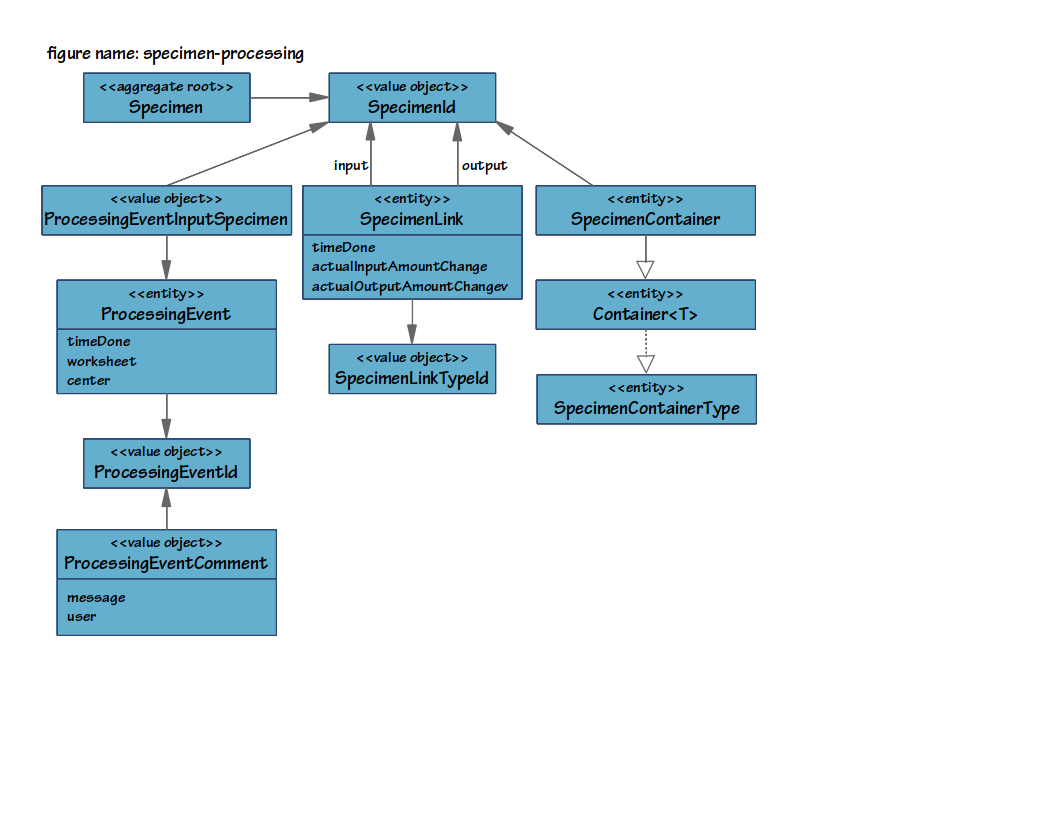
\includegraphics[trim={10mm 42mm 78mm 18mm}, clip,
    width=0.75\textwidth]{images/specimen-processing}
  \caption{Specimen Processing Model}
  \label{fig:specimen-processing}
\end{figure}

\subsection*{ProcessingEvent}
The \entitytarget{ProcessingEvent} entity records information about a group of
specimens that were processed at the same time. The processing event has the
following attributes: \compfont{timeDone} the time stamp for when the
processing took place; \compfont{worksheet} a unique identifier associated with
the processing event used to cross reference to other systems;
\compfont{centre} the processing centre where the processing is taking place.

\subsection*{ProcessingEventInputSpecimen}
It is possible that a single specimen be processed multiple
times. \entitytarget{ProcessingEventInputSpecimen} is used to record this.

\subsection*{SpecimenLink}
\entitytarget{SpecimenLink} is a record of the specimens and amounts involved
in a \entitylink{SpecimenLinkType}. This entity provides more detailed
information about the parentage of a specimen, i.e. the \compfont{input-output}
pair could be considered a parent-child relationship. This is opposed to
collection events, which provide much more general heritage information. So,
special care must be taken to ensure that \entitylink{SpecimenCollectionEvent}
and \entitylink{SpecimenLink} entities are consistent. The \compfont{output}
must be in all the same collection events as the \compfont{input}, but if two
specimens are in the same collection event they do \emph{not} need to be
associated (directly or transitively) through a \entitylink{SpecimenLink}. Also
note that the \compfont{input} does \emph{not} need to be in the same
collection event(s) as the \compfont{output}.

\subsection*{SpecimenContainer}
The container that holds this specimen. Specimen containers are containers that
only hold specimens. More information for containers is given in Chapter
\ref{containers}.

\subsection*{ProcessingEventComment}
A \entitytarget{ProcessingEventComment} contains a textual message and the
user that added the comment. The date and time the comment is made is recorded
as meta data. A processing event can have one or more comments.

% Local Variables:
% compile-command: "/usr/bin/rubber --pdf main"
% End:
